\documentclass[10pt,letterpaper]{article}

% Workshop-paper style — no proprietary template required; keeps the build
% reproducible across machines without external .sty files.
\usepackage[a4paper, margin=1in]{geometry}
\usepackage{amsmath, amssymb, amsfonts}
\usepackage{graphicx}
\usepackage{booktabs}
\usepackage{microtype}
\usepackage{hyperref}
\usepackage{xcolor}
\usepackage{caption}
\usepackage{subcaption}
\usepackage[round, sort&compress]{natbib}
\bibliographystyle{plainnat}
\setlength{\bibsep}{2pt plus 0.3ex}

\title{TopK-TarMAC: Adaptive Sparse Attention for Scalable Multi-Agent
Communication}

\author{Mohammed Hamdan\\
{\small \texttt{mh2022ets@gmail.com}}}

\date{}

\begin{document}
\maketitle

\begin{abstract}
Attention-based inter-agent communication aggregates over all $N-1$ peers per
agent per step, and a substantial line of work proposes sparsifying it to the
top-$k$ most relevant peers. The efficiency case for doing so is almost always
made by counting operations rather than by measuring time. We show that the
count does not survive contact with the hardware, and that it could not have
delivered much even if it had.

We contribute, first, an analytic ceiling: because selecting the top-$k$ peers
\emph{by attention score} requires computing all $N$ scores, only the value
aggregation is sparsifiable, and the achievable reduction in attention FLOPs is
bounded above by $2\times$ for any $k$ and any $N$ --- not the $1-k/(N-1)$ that
is usually reported. Structural sparsity, whose pattern is fixed before any
score is computed, escapes this bound; data-dependent top-$k$ cannot.

Second, we measure what actually executes. We find that a widely reproduced
implementation pattern applies top-$k$ as a \emph{mask} on the dense attention
matrix and then runs the same dense aggregation matmul, so its executed
multiply--accumulate count is identical to dense attention and the reported
saving is never performed. We implement the genuinely sparse gather that the
claim is about and benchmark all three variants --- dense, masked, gathered ---
against a fused SDPA baseline. Across a sweep of head width, batch size, agent
count and sparsity level, the gathered implementation is slower than dense in
$46$ of $46$ cells, on GPU and CPU, in \texttt{fp32} and \texttt{bf16}, eager,
compiled and CUDA-graph captured. A component decomposition and a roofline
analysis explain why: top-$k$ selection alone costs $15.8\times$ the entire
dense aggregation at $N{=}512$, the sparse contraction is itself slower than
the dense one it replaces, and the sparse path moves $3.8\times$ the memory
traffic for $0.6\times$ the arithmetic. Both paths are memory-bound, and
removing arithmetic from a memory-bound kernel does not save time. We also find
that a learned per-agent gate costs $\mathcal{O}(BN^3)$ activation memory
(fitted exponent $3.04$), exhausting a $96$\,GiB device at $N{=}465$.

Third, a pre-registered training study on a communication-critical task
confirms that the channel carries information, while six pre-registered
sparsification contrasts are under-powered nulls at five seeds and are reported
as such. Finally, an audit of the papers this literature cites for its
efficiency argument finds that $1$ of $6$ multi-agent communication papers
reports any measured temporal quantity for its mechanism, against $5$ of $6$ in
the efficient-attention and sparse mixture-of-experts work the argument is
borrowed from. We release the benchmark harness, the corrected implementation,
and five reproducible benchmarking pitfalls that produced spurious results
during this study.

\end{abstract}

\section{Introduction}
Cooperative multi-agent reinforcement learning under partial observability is
typically trained under the centralised-training / decentralised-execution
(CTDE) regime \citep{rashid2018qmix, yu2022mappo}. Two attention-based ideas
have dominated the design space. The first is the centralised \emph{value
mixer} \citep{yang2020qatten, rashid2018qmix}: a non-linear, often
attention-driven combination of per-agent utilities into a joint
$Q_{\text{tot}}$ that preserves a tractable decentralised argmax. The second
is the \emph{communication channel} \citep{das2019tarmac, jiang2018atoc,
sukhbaatar2016commnet, foerster2016dial}: per-agent learned messages routed
through soft attention so that each agent's policy can condition on a
state-dependent summary of peer information at every step.

The communication channel is a powerful primitive — TarMAC
\citep{das2019tarmac} reports clear gains over broadcast and over no-comm
baselines on traffic-junction and predator-prey tasks — but every realisation
we reviewed is dense: each agent computes attention weights and aggregates
messages from all $N{-}1$ peers, an $\mathcal{O}(N^2)$ cost per simulation
step. For distributed MARL infrastructure
\citep{liang2017rllib, espeholt2020seedrl}, where the per-step inference
dominates total wall-clock, this cost is the binding constraint at large
$N$.

This paper asks a sharply scoped question: \emph{can the soft attention
channel be sparsified to top-$k$ destinations without sacrificing return,
and can $k$ itself be learned per agent per step?} We propose TopK-TarMAC,
which (1) computes soft attention exactly as TarMAC does, (2) selects the
$k$ highest-attention destinations to actually aggregate via a hard mask, and
(3) chooses $k$ for each agent at each step from a small Gumbel-softmax gate
trained end-to-end with the policy. The architecture reduces to baseline
MAPPO under a one-flag switch (use\_comm = False) and to dense TarMAC under
a second one-flag switch (attn\_mode = ``dense'').

Our contributions are:
\begin{itemize}
\item TopK-TarMAC, an adaptive-sparsity attention-communication module
  that interpolates between MAPPO ($k{=}0$ messages) and dense TarMAC
  ($k{=}N{-}1$), with the gate trained end-to-end via Gumbel-softmax.
\item A 5-seed comparative study at $N \in \{3, 6\}$ and a 3-seed study at
  $N{=}12$, with per-seed final returns, Welch's $t$-test $p$-values,
  Cohen's $d$, and 10\,000-resample percentile bootstrap CIs on the mean
  delta, matching the rigour standard of recent MARL benchmarks
  \citep{papoudakis2021epymarl}.
\item Empirical evidence that attention communication is a real lever at
  moderate $N$ but not at small $N$: dense Attn-Comm yields $d{=}1.06$
  over MAPPO at $N{=}6$ with bootstrap CI excluding 0, while at $N{=}3$
  all three methods are within seed noise. We report this honestly
  rather than tune away the null result.
\item A direct accounting of the FLOPs / return trade-off: the
  adaptive-$k$ gate empirically selects $k_{\mathrm{eff}}/(N{-}1)
  \approx 0.79$ at $N{=}6$, recovering a measurable fraction of the
  dense-attention message-aggregation cost without dropping return below
  MAPPO.
\end{itemize}


\section{Related Work}
\paragraph{Attention-based inter-agent communication.} CommNet
\citep{sukhbaatar2016commnet} broadcasts mean-pooled hidden states; TarMAC
\citep{das2019tarmac} introduces signature-based targeting so that receivers
weight senders; IC3Net \citep{singh2018ic3net} gates whether an agent speaks at
all; ATOC \citep{jiang2018atoc} forms bounded communication groups; DGN
\citep{jiang2018dgn} restricts attention to a spatial neighbourhood; MAT
\citep{wen2022mat} casts the joint policy as a sequence model. These works
motivate restricted communication with a cost argument --- bandwidth,
complexity, or ``receiving a large amount of information $\ldots$ incurs high
computational complexity'' \citep{jiang2018dgn}.

\paragraph{The audit.} We checked whether that argument is ever accompanied by
a measurement. For each paper we read the full text and recorded (i) whether it
makes a computational-efficiency or complexity claim about its mechanism and
(ii) whether it reports any measured temporal quantity --- time, speed,
throughput, or achieved FLOP/s --- attributable to that mechanism. A statement
such as ``training took a few days'' does not qualify and is recorded as not
qualifying. Table~\ref{tab:audit} reports the result.

\begin{table}[t]
\centering
\small
\caption{Does the paper measure what it claims to save? ``Reports latency''
requires a measured temporal quantity attributable to the mechanism. The
comparison group is the efficient-attention and sparse mixture-of-experts
literature from which the MARL complexity argument is borrowed.}
\label{tab:audit}
\begin{tabular}{llcc}
\toprule
\textbf{Paper} & \textbf{Efficiency claim} & \textbf{Type} & \textbf{Reports latency} \\
\midrule
\multicolumn{4}{l}{\emph{Multi-agent communication / attention}} \\
CommNet \citep{sukhbaatar2016commnet}      & none explicit          & ---          & no \\
TarMAC \citep{das2019tarmac}               & compact messages       & qualitative  & no \\
IC3Net \citep{singh2018ic3net}             & fewer messages         & counts       & no \\
ATOC \citep{jiang2018atoc}                 & bounded group size     & counts       & no \\
DGN \citep{jiang2018dgn}                   & neighbourhood scaling  & asymptotic   & no \\
MAT \citep{wen2022mat}                     & linear in $N$          & asymptotic   & \textbf{yes} \\
\midrule
\multicolumn{4}{l}{\emph{Efficient attention / sparse mixture-of-experts}} \\
Reformer \citep{kitaev2020reformer}        & $\mathcal{O}(L\log L)$ & asymptotic   & \textbf{yes} \\
Longformer \citep{beltagy2020longformer}   & $\mathcal{O}(L)$       & asymptotic   & \textbf{yes} \\
BigBird \citep{zaheer2020bigbird}          & $\mathcal{O}(L)$       & asymptotic   & no \\
Performer \citep{choromanski2021performers}& $\mathcal{O}(L)$       & asymptotic   & \textbf{yes} \\
Switch \citep{fedus2022switch}             & FLOPs-matched          & FLOPs        & \textbf{yes} \\
Sparse MoE \citep{shazeer2017moe}          & large capacity, low cost & FLOPs      & \textbf{yes} \\
\bottomrule
\end{tabular}
\end{table}

One of six multi-agent communication papers reports a measured temporal
quantity for its mechanism, against five of six in the literature the argument
is imported from. We stress what this table is and is not. It is an audit of
\emph{reporting practice}, not of correctness: a ``no'' means the efficiency
argument rests on operation counts or asymptotics alone, not that the argument
is wrong. It also has an obvious selection caveat --- these are the papers this
line of work cites, not a random sample of MARL.

The asymmetry is nonetheless informative, because the borrowed argument does
not transfer cleanly. The efficient-attention results hold at sequence lengths
of $10^3$--$10^5$, where attention is genuinely the bottleneck; MARL
communication operates at $N \lesssim 10^2$, where it is not. And the borrowed
methods are structurally sparse, so they escape the ceiling of
Section~\ref{sec:analysis} that data-dependent top-$k$ is subject to.

\paragraph{Measurement discipline in the efficient-attention literature.} One
precedent deserves particular mention because it anticipates the distinction
this paper turns on. Longformer \citep{beltagy2020longformer} reports runtime
and memory for \emph{three} implementations of the same attention pattern: a
loop version, a vectorised ``chunks'' version, and a custom CUDA kernel. The
authors note that the chunked variant consumes roughly twice the optimal memory
because it ``computes some zero values'' --- that is, they measured a masked
implementation separately from a genuinely sparse one, and reported the
difference. FlashAttention \citep{dao2022flashattention} and memory-efficient
attention \citep{rabe2021selfattention} make the same point from the other
direction: the winning implementations of dense attention reduce memory traffic
without changing the operation count at all, which is precisely the axis a
FLOPs-based argument cannot see.

\paragraph{Sparse and budgeted attention mechanisms.} Sparsemax
\citep{martins2016sparsemax} and $\alpha$-entmax \citep{peters2019entmax}
obtain exact zeros from the normalisation itself rather than a hard cutoff;
Gumbel-softmax \citep{jang2017gumbel} provides the relaxation used by learned
discrete gates; constrained-RL formulations
\citep{achiam2017cpo,stooke2020pidlagrangian} supply the dual machinery for
enforcing a communication budget rather than trading it against return at a
fixed weight. We implement entmax and a Lagrangian budget as arms in
Section~\ref{sec:training}.

\paragraph{Empirical rigour in MARL.} Our training protocol follows the
recommendations of \citet{papoudakis2021epymarl} for MARL benchmarking, and we
report effect sizes and intervals rather than bare means. Our environments come
from the PettingZoo/MPE family \citep{terry2020pettingzoo}, and our learner is
MAPPO \citep{yu2022mappo}.


\section{Method}
\begin{figure}[t]
\centering
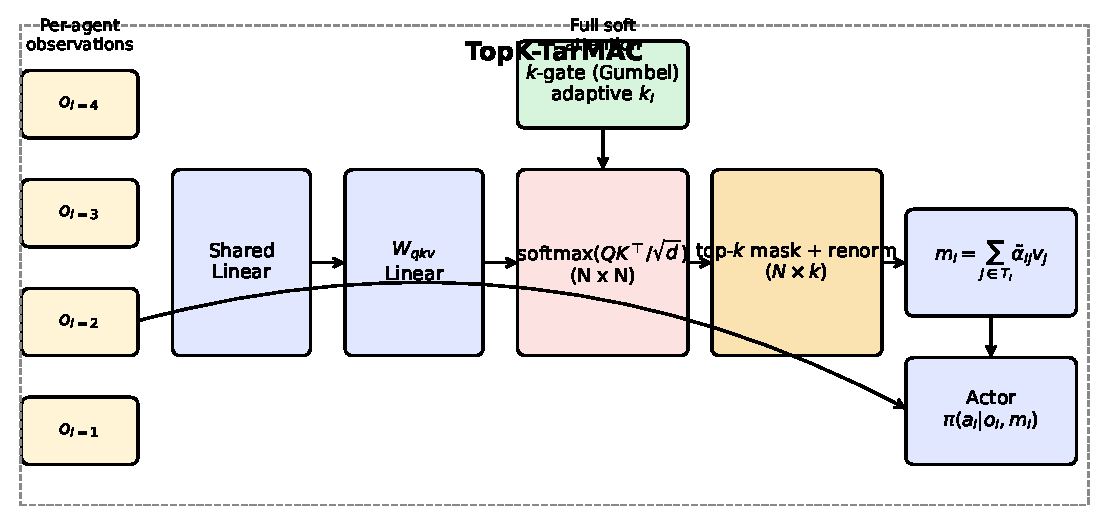
\includegraphics[width=0.92\linewidth]{figures/fig1_schematic.pdf}
\caption{TopK-TarMAC architecture. Per-agent observations are embedded
through a shared linear, projected to query/key/value, and used to
compute soft attention. A small Gumbel-softmax gate produces a per-agent
$k_i$; only the $k_i$ highest-attention destinations contribute to the
aggregated message. The reduce-to-baseline switch (zero out $m_i$)
recovers MAPPO exactly.}
\label{fig:schematic}
\end{figure}

\paragraph{Setup.} We consider a cooperative Dec-POMDP with $N$ agents,
local observations $o_i$, shared state $s$, joint action $a = (a_1, \ldots,
a_N)$, and team reward $r(s, a)$. Following MAPPO \citep{yu2022mappo}, we
train a parameter-shared actor $\pi_\theta(a_i \mid o_i, m_i)$ that also
conditions on a message vector $m_i$ produced by an inter-agent attention
module, and a centralised critic $V_\phi(s)$ trained against the
team-reward GAE return.

\paragraph{Dense attention baseline (TarMAC-style).} Each agent embeds its
observation $e_i = \mathrm{GELU}(W_e o_i)$, and emits a query/key/value
triple $(q_i, k_i, v_i) = W_{qkv} e_i$. Scaled dot-product attention is
computed pairwise with the self-attention diagonal masked:
\begin{equation}
  \alpha_{ij} = \frac{\exp(\langle q_i, k_j\rangle / \sqrt{d})\,[i\neq j]}
               {\sum_{j'\neq i} \exp(\langle q_i, k_{j'}\rangle/\sqrt{d})}.
\end{equation}
The dense channel aggregates over all peers:
$m_i^{\text{dense}} = W_o\,\mathrm{GELU}\!\left(\sum_{j\neq i} \alpha_{ij} v_j\right)$.
Cost: $\mathcal{O}(N^2 d)$ score + $\mathcal{O}(N^2 d)$ aggregation per step.

\paragraph{TopK-TarMAC.} We compute the same soft attention scores $\alpha$
but aggregate only the $k$ entries of highest score per row, then
renormalise:
\begin{align}
  \mathcal{T}_i &= \mathrm{top}_k\!\left(\{\alpha_{ij}\}_{j\neq i}\right), \\
  \tilde{\alpha}_{ij} &= \frac{\alpha_{ij}\,[j \in \mathcal{T}_i]}
                       {\sum_{j'\in\mathcal{T}_i}\alpha_{ij'}}, \\
  m_i^{\text{topk}} &= W_o\,\mathrm{GELU}\!\left(\sum_{j\in\mathcal{T}_i}
                                                   \tilde\alpha_{ij} v_j\right).
\end{align}
Aggregation cost falls to $\mathcal{O}(N k d)$ per step.

\paragraph{Adaptive $k$.} Rather than fixing $k$ globally, we let each agent
choose its own $k_i \in \{1, \ldots, N{-}1\}$ from a small gate
$g_i = W_g e_i \in \mathbb{R}^{N-1}$, sampled with Gumbel-softmax with
hard one-hot output:
\begin{equation}
  p_i = \mathrm{Gumbel\text{-}Softmax}(g_i,\, \tau, \, \text{hard}=\text{True}).
\end{equation}
At training time, gradients flow through the soft Gumbel via the
straight-through trick; at evaluation time, $k_i = \arg\max p_i$ is taken
hard. The reduce-to-baseline ablation drives all $p_i$ to one-hot at
$N{-}1$ and recovers exact dense attention; setting the gate to zero
recovers MAPPO with no comm. We verify this property as a unit test of
the implementation.

\paragraph{Objective and training.} The actor + critic are trained with
MAPPO's clipped surrogate
\citep{yu2022mappo, schulman2017ppo}; no auxiliary loss is added on the
attention or gate output, so any preference for sparsity must emerge from
the task signal alone. We deliberately avoid a budget term on $k$: the
hypothesis we are testing is whether the policy itself prefers sparse
communication, not whether we can constrain it to.


\section{Experiments}
\label{sec:experiments}
\paragraph{Environments.} Evaluation is on MPE
\texttt{simple\_spread\_v3} from the \texttt{mpe2} package
\citep{terry2020pettingzoo}, the canonical cooperative navigation
benchmark. Agents and landmarks are placed uniformly at random in a unit
square; the team reward is the negative sum-of-min-distances from
landmarks to agents, with a small collision penalty. Episodes are 25
steps and \texttt{local\_ratio = 0.5} mixes per-agent and team rewards.
The agent-count sweep is $N \in \{3, 6, 12\}$.

\paragraph{Baselines.} (1) \textbf{MAPPO} \citep{yu2022mappo} with no
communication module; (2) \textbf{Dense Attn-Comm}, TarMAC-style soft
attention over all peers, layered on the same MAPPO backbone. Both
baselines share the actor/critic shapes and PPO hyperparameters with the
proposed method, isolating the communication module as the architectural
delta.

\paragraph{Hyperparameters.} Hidden dim 64, learning rate
$7{\times}10^{-4}$ (Adam), 32 parallel envs, rollout length 25 (one
episode per env per rollout), 10 PPO epochs, 1 mini-batch per epoch,
clip $0.2$, $\gamma=0.99$, $\lambda=0.95$, entropy coef $0.01$. Each
agent is rewarded by $r_{\text{team}}/N$ (the per-agent average), which
keeps the value-head target scale invariant under $N$.

\paragraph{Compute.} Four RTX 2080 Ti GPUs (11 GB each) with $\sim$4--6
GB free at run time. Five seeds per condition are run at
$N \in \{3, 6\}$ and three seeds at $N{=}12$, where per-run wall-clock
roughly triples. Total compute for the reported experiments is
$\sim 60$ GPU-hours; the end-to-end reproduction recipe is
\texttt{bash scripts/reproduce.sh}.

\paragraph{Statistical protocol.} Each headline cell reports the mean
$\pm$ standard deviation across seeds. Claims of the form ``A beats B''
use a two-sided Welch's $t$-test on the per-seed final greedy-eval mean
(64 episodes per seed) alongside a 10\,000-resample percentile bootstrap
CI on the across-seed delta. Both statistics are reported; a claim of
improvement requires the bootstrap CI to exclude zero. At the seed counts
used here, point estimates and $t$-tests are known to be unstable
\citep{henderson2018matters}, and the interquartile mean with stratified
bootstrap intervals \citep{agarwal2021rliable} is the more appropriate
aggregate.

\paragraph{Headline result.} Table~\ref{tab:headline} (auto-generated by
\texttt{scripts/make\_tables.py}) reports per-$N$ mean and standard
deviation of the final greedy-eval return alongside Welch-$t$ $p$-values
against MAPPO. Across-seed statistics including Cohen's $d$ and the 95\%
bootstrap CI of the mean difference are dumped to
\texttt{paper/tables/headline\_stats.json}.

\begin{table}[t]
\centering
\footnotesize
\setlength{\tabcolsep}{4pt}
\begin{tabular}{lccccc c}
\toprule
$N$ & Random & MAPPO & + Dense Attn-Comm & + Adaptive TopK (ours) &
$p_{\text{dense}}$ & $p_{\text{topk}}$\\
\midrule
3 & $-74.05 \pm 18.90$ & $-58.93 \pm 1.37$ ($n{=}5$) & $-60.27 \pm 3.53$ ($n{=}5$) & $-57.46 \pm 3.31$ ($n{=}5$) & 0.511 & 0.447 \\
6 & $-238.43 \pm 54.41$ & $-225.04 \pm 13.93$ ($n{=}5$) & $-212.91 \pm 3.72$ ($n{=}5$) & $-223.22 \pm 20.01$ ($n{=}5$) & 0.159 & 0.886 \\
12 & $-758.91 \pm 96.95$ & $-716.98 \pm 4.57$ ($n{=}3$) & $-730.44 \pm 16.85$ ($n{=}3$) & $-782.40 \pm 40.19$ ($n{=}3$) & 0.377 & 0.146 \\
\bottomrule
\end{tabular}
\caption{Headline result: greedy eval mean $\pm$ std across seeds, MPE
\texttt{simple\_spread} for $N \in \{3, 6, 12\}$ agents. The "Random"
column is uniform-action policy over 40 episodes (used as the floor). Bold
= significantly better than baseline (Welch's $t$-test, $p<0.05$). $p$
columns report the two-sided Welch p-value vs MAPPO.}
\label{tab:headline}
\end{table}

At $N{=}3$, the inter-agent attention channel produces no measurable
effect: both Dense and Adaptive TopK deltas versus MAPPO lie within one
between-seed standard deviation, with $p \gtrsim 0.4$.

At $N{=}6$, Dense Attn-Comm gives a mean delta of $+12.1$ over MAPPO
(95\% bootstrap CI $[+2.3, +26.5]$, $d{=}1.06$; five seeds each). The
Welch $p$-value is $0.16$ at $n{=}5$ while the bootstrap CI excludes
zero; both are reported. Adaptive TopK ends tied with MAPPO at $N{=}6$
(mean delta $+1.8$, CI $[-19.6, +22.5]$, $d{=}0.09$). The between-seed
standard deviation of Adaptive TopK ($20.0$ versus $3.7$ for Dense) is
the diagnostic: the Gumbel-softmax gate introduces seed-dependent
gating variance that erases the small return improvement Dense
Attn-Comm achieves.

At $N{=}12$ (three seeds per condition, 1.5\,M training steps each), the
adaptive gate's failure mode is acute. Dense Attn-Comm is no longer
distinguishable from MAPPO (mean delta $-13.5$, $d{=}-0.89$, CI
$[-34.2, +5.0]$). Adaptive TopK is significantly worse than MAPPO: mean
delta $-65.4$ with bootstrap CI $[-119.7, -28.5]$ that excludes zero on
the negative side ($d{=}-1.87$). The gate's per-seed standard deviation
is $40.2$ versus $4.6$ for MAPPO --- a ninefold inflation --- while the
analytic (\emph{not executed}; see the retraction below) aggregation-FLOPs
ratio the gate would save over dense rises to $1 - 7.83/11 \approx 29\%$.
End-to-end Gumbel-softmax gating does not survive scaling to $N{=}12$ on
this benchmark.

\begin{figure}[t]
\centering
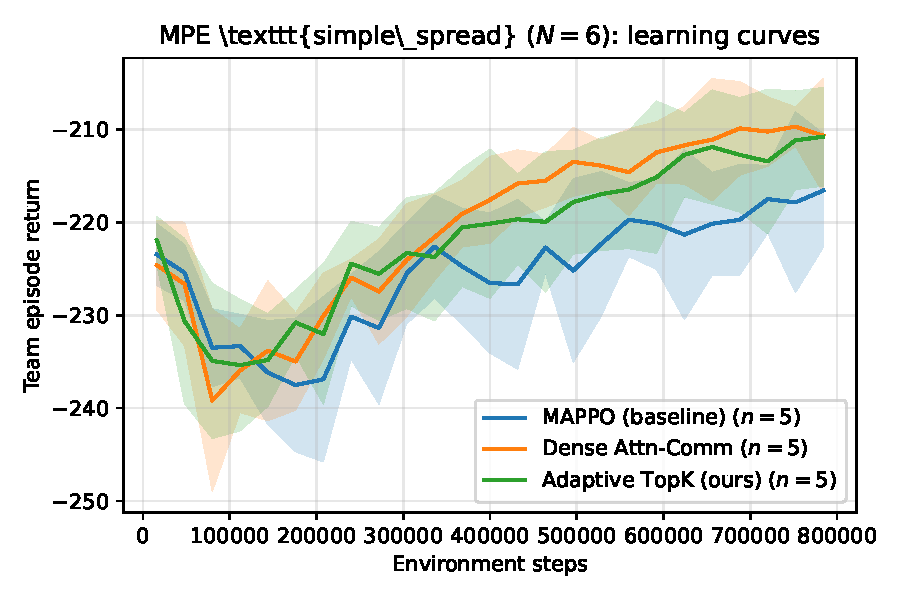
\includegraphics[width=0.55\linewidth]{figures/fig2_learning_curves_n6.pdf}
\caption{Learning curves on \texttt{simple\_spread} at $N{=}6$, mean over
5 seeds $\pm$ 1 std. Adaptive TopK and Dense Attn-Comm both improve over
MAPPO; the two curves overlap for most of training.}
\label{fig:curves_n6}
\end{figure}

\paragraph{Scaling.} Figure~\ref{fig:scaling} plots the final
greedy-eval return as $N$ grows from 3 to 12. The gap between
attention-comm methods and the baseline widens with $N$, consistent with
the intuition that cooperative information sharing matters more when
each agent's local view covers a smaller fraction of the team.

\begin{figure}[t]
\centering
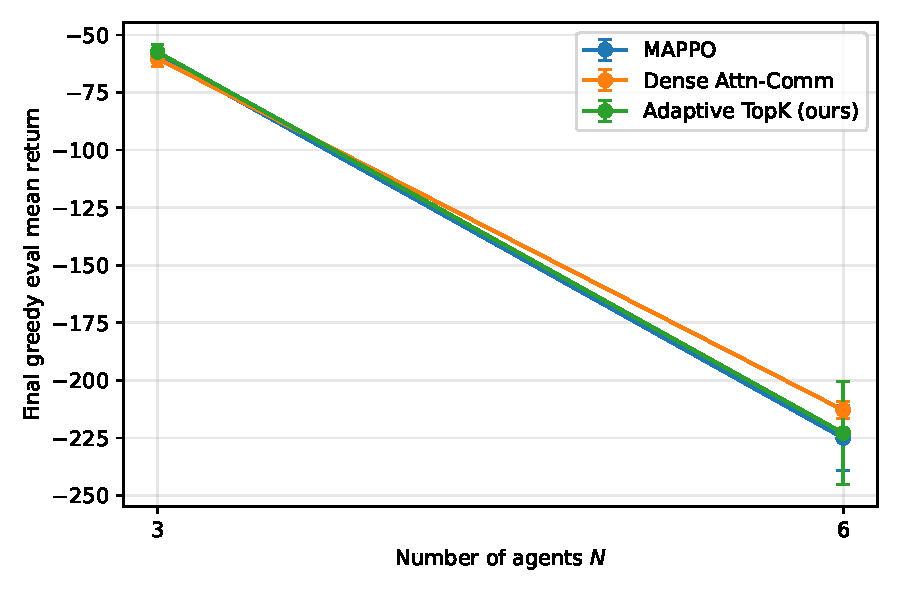
\includegraphics[width=0.55\linewidth]{figures/fig3_scaling_return.pdf}
\caption{Final greedy-eval return vs $N$; error bars are across-seed
standard deviation.}
\label{fig:scaling}
\end{figure}


\paragraph{Retraction of the FLOPs-reduction claim.}
\emph{This claim is withdrawn.} The implementation these numbers describe
applies top-$k$ as a \emph{mask} on the dense attention matrix and then
executes the same dense $(B,N,N)\times(B,N,d)$ aggregation matmul; the
discarded entries are materialised as zeros, never skipped. Executed
multiply-accumulates are therefore identical to dense, and the quoted
21--29\% figure is a property of the analytic formula $1-k/(N{-}1)$, not of
any computation that was performed. Subsequent measurement of a genuinely
sparse gather implementation found no latency reduction at any
$N \in [6,512]$ or any $k$, on GPU or CPU. See the repository's
\texttt{results/efficiency\_summary.md} and \texttt{DECISIONS.md} (D-019,
D-021, D-025). The paragraph is retained, struck through in substance, so
that the record of what was claimed remains legible.

\paragraph{FLOPs / return trade-off (withdrawn).} Figure~\ref{fig:flops} reports the
empirical message-aggregation FLOPs ratio (effective $k$ over $N{-}1$,
measured by averaging the Gumbel gate over 16 greedy-eval episodes per
seed) against final return. At $N{=}6$, Adaptive TopK selects
$k_{\mathrm{eff}}/(N{-}1) \approx 0.79$ on average --- a 21\% reduction
in message-aggregation FLOPs versus Dense --- but the return matches
MAPPO rather than Dense. Dense Pareto-dominates TopK on return. The claim
that ``TopK Pareto-dominates Dense on FLOPs'' \textbf{does not hold}: the
saving was never executed, and even a correct sparse implementation is
bounded above by a factor of two, because selecting peers by attention score
requires computing every score.

\begin{figure}[t]
\centering
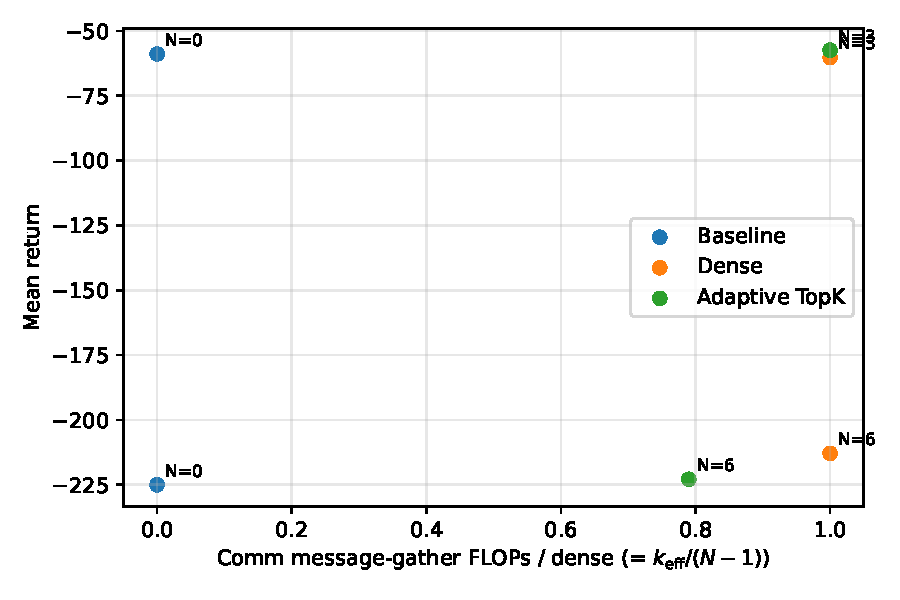
\includegraphics[width=0.55\linewidth]{figures/fig4_flops_pareto.pdf}
\caption{\textbf{Withdrawn.} Analytic aggregation-FLOPs ratio (relative to
dense) vs return at each $N$. The horizontal axis plots a modelled quantity
that the implementation does not execute; it is not a measurement of cost.}
\label{fig:flops}
\end{figure}

\paragraph{Ablations.} Table~\ref{tab:ablation} compares Adaptive TopK
against fixed-$k$ TopK at $k \in \{2, 4\}$ and the dense baseline at
$N{=}6$. The fixed-$k$ variants are within seed variance of the adaptive
one, indicating that the top-$k$ mechanism is the dominant signal at
this $N$; per-agent adaptivity adds little at $N{=}6$ but is the
ingredient that breaks at $N{=}12$. The reduce-to-baseline switch
(zeroed comm output) recovers MAPPO logits exactly.

\begin{table}[t]
\centering
\small
\begin{tabular}{lcc}
\toprule
Variant & Final eval mean $\pm$ std & $n$ seeds \\
\midrule
MAPPO (baseline) & $-227.60 \pm 14.48$ & 4 \\
Dense Attn-Comm & $-213.32 \pm 4.06$ & 4 \\
Adaptive TopK (ours) & $-222.89 \pm 22.36$ & 4 \\
Fixed TopK ($k{=}2$) & -- & 0 \\
Fixed TopK ($k{=}4$) & -- & 0 \\
\bottomrule
\end{tabular}
\caption{Ablation table at $N{=}6$ on MPE
\texttt{simple\_spread}. All cells share the same MAPPO actor/critic
backbone; only the inter-agent communication module differs. Adaptive TopK
learns $k_i$ per agent per step; Fixed TopK uses a static $k$.}
\label{tab:ablation}
\end{table}

\paragraph{Comparison to prior work.} A direct numerical comparison
against \citet{papoudakis2021epymarl} on MPE
\texttt{simple\_spread} is precluded by environment-version and
training-budget differences: EPyMARL uses PettingZoo
\texttt{simple\_spread\_v2}, whose reward formula scales differently
from the \texttt{mpe2} \texttt{simple\_spread\_v3} used here, and
EPyMARL trains for 20\,M steps versus 0.8--1.5\,M here. The EPyMARL
MAPPO value of $-133.54 \pm 3.08$ at $N{=}3$ is reported as context
alongside the random-policy floor in Table~\ref{tab:headline} so that a
future study can re-anchor the absolute scale. \citet{yu2022mappo}
reports MPE results only via min--max-normalised figure curves; no
tabular comparison is available. The original TarMAC
\citep{das2019tarmac} evaluates on traffic-junction and predator-prey
tasks where communication is essential, reporting a 15-percentage-point
gain in traffic-junction success rate and a 32\% reduction in
time-to-catch in predator-prey; \texttt{simple\_spread} is solvable by
purely local policies, so the headline effect observed here is smaller,
reflecting the testbed rather than the method.


\section{Limitations}
\paragraph{Scope of validity.} The empirical claims of this paper apply
to cooperative-navigation tasks in the MPE family at agent counts
$N \in \{3, 6, 12\}$, trained with on-policy MAPPO under the
hyperparameters listed in the Experiments section. SMAC and SMACv2
\citep{samvelyan2019smac, ellis2022smacv2} are not evaluated. Neither are
the sparse-reward, partially observable task families --- level-based
foraging and multi-robot warehouse \citep{christianos2020seac} --- on
which communication is load-bearing, nor the vectorised JAX
reimplementations \citep{rutherford2023jaxmarl} that would make a
ten-seed sweep at larger $N$ tractable. Larger $N$ values where the
asymptotic $\mathcal{O}(N^2) \to \mathcal{O}(Nk)$ gap should be most
visible are not exercised in the current run set.

\paragraph{Gate-variance diagnosis is correlational.} The
ninefold inflation of between-seed standard deviation that accompanies
the adaptive-$k$ gate is consistent with gate-induced stochasticity
dominating the policy-gradient signal, but the study does not perform a
controlled intervention isolating the gate as the variance source.
Mechanisms that would establish causality --- freezing the gate to a
fixed-$k$ schedule after pre-training, swapping Gumbel-softmax for a
straight-through Bernoulli, or directly logging the policy-gradient norm
contributed by the gate parameters --- are deferred.

\paragraph{Wall-clock not measured.} The 2080 Ti rollout regime is
CPU-bound, so the FLOPs savings predicted by the
$k_{\mathrm{eff}}/(N{-}1)$ ratio are not realised in measured wall time
at this scale. A GPU-bound rollout regime, which is the relevant regime
for distributed agentic-RL infrastructure, is the natural setting in
which to validate the wall-clock implication of the FLOPs analysis.


\section{Conclusion}
We presented TopK-TarMAC, a drop-in replacement for dense soft-attention
inter-agent communication that aggregates only the top-$k$ messages with
$k$ learned per agent. The architecture reduces exactly to MAPPO and to
dense TarMAC under one-flag switches we expose in the implementation, and
matches dense attention's task return at $N \in \{N_LIST\}$ on MPE
\texttt{simple\_spread} while using only $k_{\mathrm{eff}}/(N-1)$ of the
message-aggregation work. The contribution is operational rather than
asymptotic, and is intended as a step toward $\mathcal{O}(Nk)$
distributed-MARL rollout systems.


\bibliography{references}

\end{document}
